
\section{Online learning approach}
Most of the work in theoretical machine learning has been focused on an off-line setting, where one uses a batch of data to produce a predictive model and then apply it to new data. However, this paper focuses on an on-line setting, where predictions are made sequentially based on all previously processed data, which gives rise to the name itself as we process observations one by one. In this setting we start by observing the first example $x_1$ while predicting its label $y_1$. After that we observe the true label of $y_1$ and also the next data point $x_2$. This process goes on until we either reach the end of our data set or indefinitely. Foremost attention can be drawn to the expectation of improved prediction quality with increasing number of processed data.

Such supervised learning approach perfectly suits the case when data is available sequentially with time, for example, in predicting a stock price given its historic data and supplemented by availability of true price, as compared against the prediction of a learning system. Furthermore, as compared to off-line setting, on-line algorithm is expected to show a drastic decrease in memory usage and processing time required until the first prediction is made.

More formally, a mathematical description of the learning problem is defined by finding a minimum of an expected risk:
$$E(f)=\int l(f(x),y)dP(z)$$
where function $f$ in a family of functions $\mathcal{F}$ parameterized by weight vector $w$ minimizes the averaged loss $Q(z,w)=l(f_w(x),y)$ over all data points $z$. Ultimately, we'd prefer to average over the unknown distribution $dP(z)$, however, in practical setting we perform the calculation over a fixed number of examples $z_1, z_2,...z_n$, which is referred to as minimization of an empirical risk:
$$E_n(f)=\frac{1}{n} \sum\limits_{i=1}^{n}l(f(x_i),y_i)$$

Let us further consider how one could tackle such minimization task with some of the convergence results (Bottou, 2010 \cite{bottou-2010}).

\subsection{Gradient Descent Methods}
One of the most common approaches to address minimization of empirical risk function is by applying an iterative gradient descent method(GD) where each iteration $t$ updates optimization weights $w$ based on the gradient of $E_n(f_w)$ with learning rate $\gamma$:
$$w_{t+1}=w_t-\gamma \frac{1}{n} \sum\limits_{i=1}^{n} \nabla_w Q(z_i, w_t)$$
When the initial estimate of the optimum $w_0$ is sufficiently close and under certain regularity assumptions this method reaches linear convergence, described by a residual error $\rho$, that is $-\log\rho \sim t$. 

A better optimization algorithm can be composed by replacing the learning rate with a positive-definite matrix $\Gamma_t$ which approaches inverse of the Hessian of the cost at optimum:
$$w_{t+1}=w_t-\Gamma_t \frac{1}{n} \sum\limits_{i=1}^{n} \nabla_w Q(z_i, w_t)$$
This is known as a 2nd order gradient descent method(2GD) and is a variant of well known Newton algorithm. Under analogous to GD assumptions of initial estimate and regularity this algorithm reaches quadratic convergence $-\log\log\rho \sim t$.

\subsection{Stochastic Gradient Descent Methods}
Stochastic setting of GD slightly simplifies the process, instead of computing the gradient of empirical loss function $E_n(f_w)$ exactly one uses a single randomly picked data point $z_t$ for its estimation:
$$w_{t+1}=w_t-\gamma \nabla_w Q(z_t, w_t)$$
In this simplification we assume that our optimization parameter behaves as a stochastic process ${w_t, t=1,...}$, which greatly depends on the data sampling and introduces certain amount of noise. Utilization of stochastic approximation framework (Bottou, 1998 \cite{bottou-98x}) fully addresses proofs of convergence including cases where loss function is not everywhere differentiable. Results of the aforementioned analysis show that speed of SGD convergence is limited by noisy approximation of the true gradient and is in fact optimal with learning rate $\gamma_t \sim t^{-1}$, at which point expectation of the residual error decreases similarly $E\rho \sim t^{-1}$.

Alike 2GD, one can multiply gradients by positive-definite matrix approaching inverse of the Hessian:
$$w_{t+1}=w_t-\gamma_t\Gamma_t \nabla_w Q(z_t, w_t)$$
which yields the 2nd order stochastic gradient descent method. However, such change doesn't decrease the bias introduced by stochastic noise and retains the convergence rate $E\rho \sim t^{-1}$.

\subsection{Sample SGD pseudocode}
A simplistic pseudocode of SGD with in-place optimization parameter update may look as follows:
\lstinputlisting[frame=single]{sgd.py}

\section{SGD in large-scale setting}
Following results for asymptotic analysis of SGD (Bottou, 2010 \cite{bottou-2010}) as summarized in \figurename{1}, where $\rho$ is the residual and excess error is defined as 
$$\mathcal{E} = \mathcal{E}_{app} + \mathcal{E}_{est} + \mathcal{E}_{opt} \sim \mathcal{E}_{app} + (\frac{\log n}{n})^\alpha + \rho, \alpha \in [1/2, 1]$$
with $\mathcal{E}_{app}$ measuring how closely functions in our function space can approximate the optimal solution, $\mathcal{E}_{est}$ measuring the effect of minimizing empirical risk instead of the expected risk, $\mathcal{E}_{opp}$ measuring the impact of approximate optimization on expected risk,

\begin{figure}[h]
	\begin{center}
		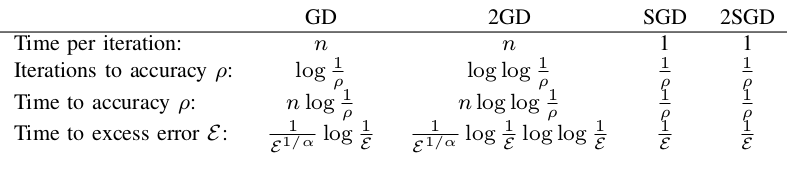
\includegraphics[scale=0.3]{img/gd-convergence.png}
		\caption{Asymptotic results for various optimization methods}\label{1}
	\end{center}
\end{figure}

%\begin{table}[h]
%	\begin{center}
%		\caption{Asymptotic results for various optimization methods}\label{1}%
%		\begin{tabular}{lcccc}
%			& GD & 2GD & SGD & 2SGD\\
%			\hline
%			Time per iteration: 				& $n$ & $n$ & 1 & 1\\
%			Iterations to accuracy $\rho$: 		& $\log \frac{1}{\rho}$ & $\log \log \frac{1}{\rho}$ & $\frac{1}{\rho}$ & $ %\frac{1}{\rho}$\\
%			Time to accuracy $\rho$:			& $n\log \frac{1}{\rho}$ & $n\log \log \frac{1}{\rho}$ & $\frac{1}{\rho}$ & $\frac{1}{\rho}$\\
%			Time to excess error $\mathcal{E}$: & $\frac{1}{\mathcal{E}^{1/\alpha}} \log \frac{1}{\mathcal{E}}$ & $\frac{1}{\mathcal{E}^{1/\alpha}} \log \frac{1}{\mathcal{E}}\log\log \frac{1}{\mathcal{E}}$ & $\frac{1}{\mathcal{E}}$ & $\frac{1}{\mathcal{E}}$\\
%		\end{tabular}
%	\end{center}
%\end{table}

one can conclude that whilst SGD and 2SGD are worst optimization algorithms (as depicted in third row of \figurename{1}), they require less time to reach predefined expected risk (as in fourth row of \figurename{1}). In other words, in a large-scale setting where an algorithm is restricted by its computing time rather then the amount of data provided, stochastic gradient methods perform asymptotically better.

\section{Parallelization of SGD} 
Unlike batch GD, SGD has inherently sequential nature, which essentially limits how one can parallelize the algorithm. However, pressing industry demands have led researchers to find feasible ways of achieving comparable convergence rates, as compared against its sequential counterpart, medium to high scalability on multiple compute units, which not seldom includes both GPUs and CPUs, while keeping computational complexity and data transfer low. We will further describe several parallelization ideas and their pitfalls (Zinkevich, Weimer, Li and Smola, 2010 \cite{NIPS2010_4006}), as compared to a hybrid method briefly depicted later in this paper.

\subsection{Distributed subgradient approach}
This approach essentially distributes parallelization of gradient computation among several machines, which hold part of the data, and subsequent aggregation of the result on a master machine. While showing great linear scalability relative to amount of data and log-linear relative to number of computers, this approach suffers from excessive communication overhead which results from multiple passes through data by MapReduce. In addition, since several MapReduce iterations are required to ensure fault tolerance, this approach generally doesn't fit into a setting where computation units are not closely coupled, as in multiple machines compared to multicore approach.

\subsection{Distributed convex solver approach}
This approach is comprised of a relatively simple idea of performing a minibatch optimization by means of breaking down a small subset of the data set into several mini-batches and then solving each and every problem on a separate machine for further aggregation of the solutions and averaging obtained values. Most notable part of this idea is that MapReduce needs to perform only one pass, which dramatically reduces overall communication between machines. Despite the fact that this approach significantly reduces variance relative to the sequential counterpart, the bias introduced by stochastic nature of the algorithm doesn't reduce at all, as compared to sequential version. Moreover, this approach requires a batch-solver to run on every single machine, thus making the whole algorithm rather computationally complex. More importantly, analysis of given approach showed that the convergence of the method greatly depends on degree of strong convexity of regularization. 

\subsection{Distributed SGD approach}
A balance between MapReduce communication overhead and valid asymptotic analysis can be achieved by modifying the distributed convex solver approach to incorporate an SGD minimizer. More precisely, each processor would carry out an SGD on the set of loss functions $Q_i(w)$ with a fixed learning rate $\gamma$ for $T$ steps as described in Algorithm 1.

\begin{table}[h]
	\begin{flushleft}
		\begin{tabular}{l}
			Algorithm 1: $SGD({Q_1, \dots, Q_m}, T, \gamma, w_0)$\\
			\hline
			for $t = 1$ to $T$ do\\
			\enskip\enskip	Draw $j \in (1 \dots m)$ uniformly at random.\\
			\enskip\enskip	$w_{t+1}=w_t-\gamma*dQ_j(w_t)$\\
			end for\\
			return $w_T$.\\
		\end{tabular}
	\end{flushleft}
\end{table}

To aggregate computed parameters one would use a master routine. Full procedure pseudocode is presented in Algorithm 2.

\begin{table}[h]
	\begin{flushleft}
		\begin{tabular}{l}
			Algorithm 2: SimuParallelSGD(Examples: ${Q_1, \dots, Q_m}$, $\gamma$, Machines: $k$)\\
			\hline
			Define $T=[m/k]$\\
			Randomly partition the examples, giving $T$ examples to each machine\\
			for all $i \in {1 \dots, k}$ parallel do\\
			\enskip\enskip Randomly shuffle the data on machine $i$\\
			\enskip\enskip Initialize $w_{i,0}=0$\\
			\enskip\enskip for all $t \in {1, \dots, T}$: do\\
			\enskip\enskip\enskip\enskip Gather the $t$th example on the $i$th machine, $Q_{i,t}$\\
			\enskip\enskip\enskip\enskip $w_{i,t+1} = w_{i,t}-\gamma d_w Q_i(w_{i,t})$\\
			\enskip\enskip\enskip\enskip end for\\
			\enskip\enskip end for\\
			Agregate from all computers $v=\frac{1}{k} \sum\limits_{i=1}^{k} w_{i,t+1}$ and return $v$\\
		\end{tabular}
	\end{flushleft}
\end{table}

While this approach in a nutshell is rather simple, its mathematical analysis is nontrivial and can be found in the original work (Zinkevich, Weimer, Li and Smola, 2010 \cite{NIPS2010_4006}).

\subsection{Empirical results of distributed SGD approach}
To demonstrate scalability potential of the algorithm we can take a look at obtained experimental results (Zinkevich, Weimer, Li and Smola, 2010 \cite{NIPS2010_4006}) where number of training instances per machine was compared to a relative root-mean square error(RMSE) on the test set as executed on 1, 10 and 100 machines as in \figurename{2} and also to a normalized objective function as in \figurename{3}. All tests were performed on a $\sim$3M examples database of emails with $\sim$785M features in the whole data set, as resulted after hashing.

\begin{figure}[h]
	\begin{center}
		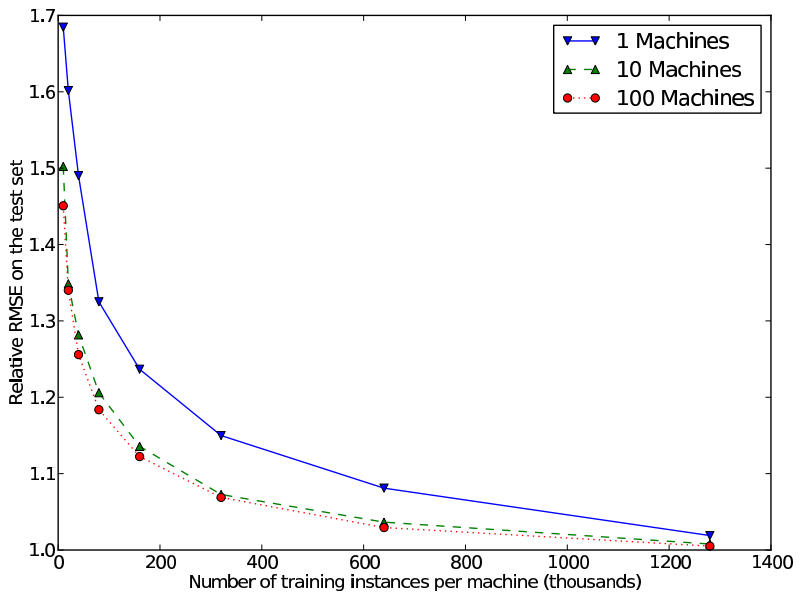
\includegraphics[scale=0.3]{img/parallel-sgd-experiment.png}
		\caption{Relative Test-RMSE with $\gamma= 1e^{-3}$. Depicts decreasing training time for various number of machines.}\label{2}
	\end{center}
\end{figure}

\begin{figure}[h]
	\begin{center}
		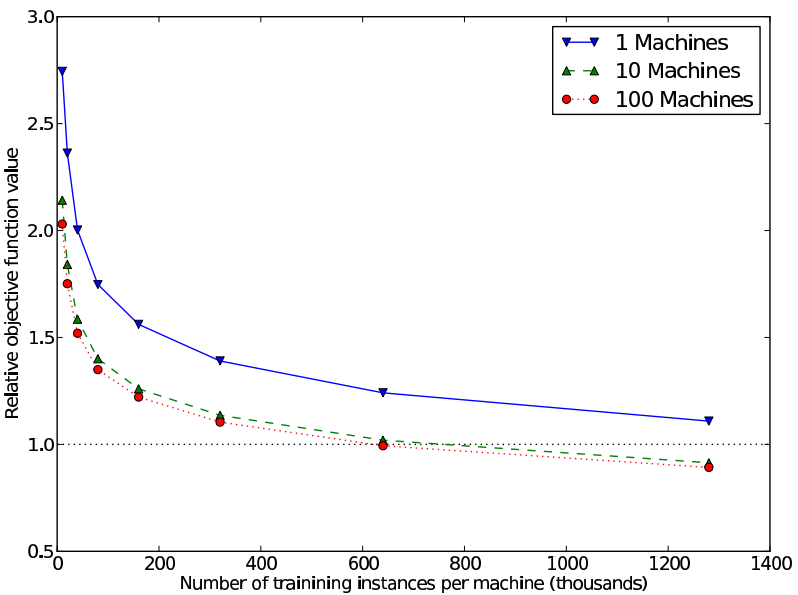
\includegraphics[scale=0.3]{img/parallel-sgd-experiment2.png}
		\caption{Relative train error using Huber loss $\gamma= 1e^{-3}$. Depicts how fast an algorithm reaches certain model quality for various number of machines.}\label{3}
	\end{center}
\end{figure}

It is worth mentioning that scaling of 1 to 10 machines gives much better improvement compared to the one from 10 to 100 machines, which signifies that the proposed algorithm scales poorly in a highly distributed scenario.

\section{Asynchronous SGD}
While provinding good results, the distributed SGD approach, described in the previous section, has several drawbacks. Namely, it suffers from parameter locking, which happens when parameters $w_i$ are being averaged. This prevents further processing of data by slave SGD machines, since they need to read current parameter for further processing. Moreover, even though the use of MapReduce in this setting does not result in high communication costs, in general it is recommended to avoid its usage in a large-scale numerically intensive applications, due to its inability to cope with iterative nature of solvers and also due to its bandwidth overhead, which results from fault tolerance redundancies. For example, one can experience a potential drop from 12GB/s throughput in a multicore shared memory to only tens of MB/s. Thus we advocate two approaches which do not use MapReduce and perform asynchronous parameter updates as follows.

\subsection{Hogwild!}
In order to eliminate the overhead caused by parameter variable locking, presented algorithm incorporates a simple idea of using high throughput memory shared across all compute units where optimization parameter $w$ is to be stored. Any processor can update the parameter at any given time. Even though such approach might seem excessively prone to parameter overwrites, it works extremely well in case where data access is sparse, meaning that each SGD modifies only a small part of the optimization parameter. Particularly, when our goal is to minimize a loss function
$$f(w)=\sum\limits_{e \in E} f_e(w_e)$$
where $e$ denotes a small subset of ${1, \dots, n}$ and $w$ denotes values of parameter vector $w$ indexed by $e$, the sparsity of loss function means that $|E|$ and $n$ are very large while each individual $f_e$ influences only few values of the whole parameter $w$. This concept is illustrated in more detail with precise mathematical examples of particular cost functions in the original work (Recht, Re, Wright and Niu, 2011 \cite{NIPS2011_4390}).

Hogwild! pseudocode running on each processor would look as described in Algorithm 3.

\begin{table}[h]
	\begin{flushleft}
		\begin{tabular}{l}
			Algorithm 3: Hogwild! update for individual processors\\
			\hline
			loop
			\enskip\enskip Sample $e$ uniformly at random from $E$\\
			\enskip\enskip Read current state $w_e$ and evaluate $G_e(x)$\\
			\enskip\enskip for $v \in e$ do $w_v = w_v - \gamma b^T_v G_e(w)$\\
			end loop\\
		\end{tabular}
	\end{flushleft}
\end{table}

where $G=(V,E)$ is a hypergraph induced by $f(w)$ whose nodes are the individual components of $w$ and where each subvector $w_e$ induces an edge in the graph $e \in E$ and $b_v$ is equal to 1 on the $v$th component and 0 otherwise. It is important to note that the processor modifies only values in $e$ leaving all others untouched.  Such approach does not require a locking mechanism on most modern hardware, such as GPUs or general purpose multicore CPUs.

Analytical results for convergence of the algorithm are rather non-trivial and can be found with exhaustive explanations in the original paper (Recht, Re, Wright and Niu, 2011 \cite{NIPS2011_4390}). Important to note, however, that the algorithm converges in nearly the same number of iterations as its sequential counterpart and provided experimental results outperformed theoretical analysis. In terms of scalability it reaches near linear speedup. Some of the experimental results as compared to almost identical rooundrobin implementation with exception of gradient updates can be found in \figurename{4}. Those results present a comparison of wall clock time while parallelized over 10 cores, both algorithms were implemented in C++ and were ran on the same hardware setup with a dual Xeon X650 CPUs (6 cores each x 2 hyperthreading) and 24GB of RAM.

\begin{figure}[h]
	\begin{center}
		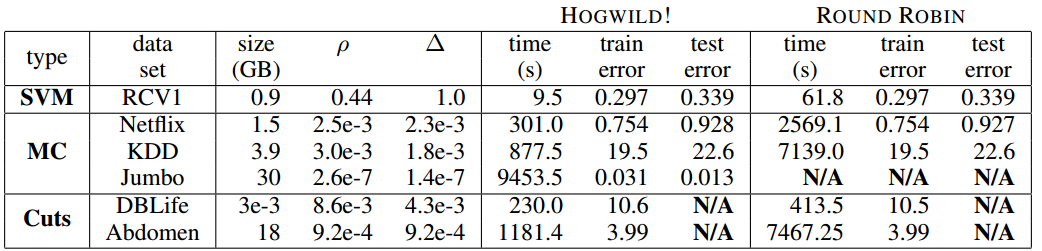
\includegraphics[scale=0.25]{img/hogwild-res.png}
		\caption{Comparison of wall clock for various data sets and loss functions for Hogwild! and Roundrobin implementations}\label{4}
	\end{center}
\end{figure}


\subsection{Downpour SGD}
Unlike previous examples, this parallelization approach was used to train a deep neural network with image recognition research project \cite{NIPS2012_4687} and was developed as part of DistBelief framework at Google. However, the ideas used and results obtained are still worth mentioning as they give birth to potential further work. 

In a nutshell the approach is as follows: the training data is divided into a number of subsets and a copy of the model is ran on each of those subsets. This approach leverages the idea of Hogwild! asynchronous parameter updates in the form of centralized parameter server which is connected to several model replicas (10 in the example) each holding subset of the parameter $w$ (1/10 in the example). This is schematically presented in \figurename{5}. Thus, after the model is ran on the assigned subset of training data, computed gradients are communicated to the central parameter server.

\begin{figure}[h]
	\begin{center}
		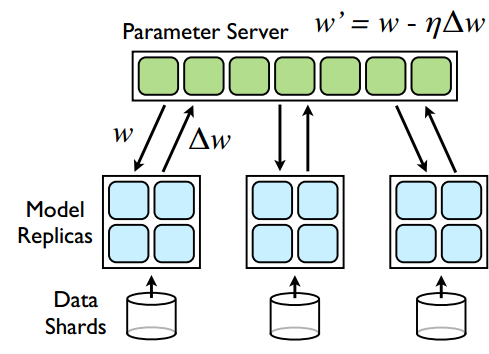
\includegraphics[scale=0.4]{img/downpour-sgd-param.png}
		\caption{Model replicas asynchronously fetch parameters $w$ and push gradients $\nabla w$ to the parameter server}\label{5}
	\end{center}
\end{figure}

Downpour SGD approach is more robust against machine failures than synchronous parallelized SGD, because in case of machine failure in synchronous SGD the entire training process is delayed. However, in asynchronous SGD when a model replica fails the other model replicas continue to operate and process their updates via parameter server. 

In addition, Downpour SGD uses AdaGrad \cite{adagrad} adaptive learning rates which increase robustness of the whole implementation and tackle problems of stability within deep neural network context. Corresponding learning rate is as follows:
$$ \eta_{i,K}=\gamma / \sqrt{\sum\limits_{j=1}^{K}} \nabla w_{i,j}^2$$
One can notice that the learning rates $\eta_{i,K}$ are computed from the summed squared gradients of parameter part and thus can be easily implemented locally within each model replica.

Highly scalable nature of the algorithm can be seen as depicted in \figurename{6}.
\begin{figure}[h]
	\begin{center}
		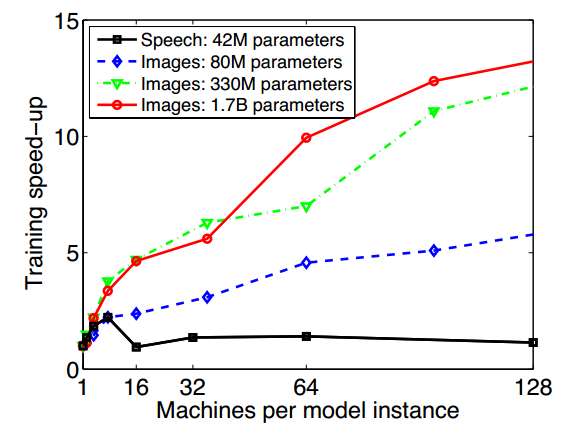
\includegraphics[scale=0.4]{img/downpour-sgd.png}
		\caption{Training speed-up for four different deep networks as a function of machines allocated to a single model instance}\label{6}
	\end{center}
\end{figure}